\documentclass[10pt,letterpaper]{report}
\usepackage{enumitem}
\usepackage[utf8]{inputenc}
\usepackage[spanish]{babel}
\usepackage{graphicx}
\usepackage{amsmath}
\usepackage{amsfonts}
\usepackage{amssymb}
\usepackage{makeidx}
\usepackage[usenames]{color}
\usepackage[left=2cm,right=2cm,top=1.5cm,bottom=1.5cm]{geometry}
\usepackage{subfiles}
\usepackage[ruled, vlined, lined, linesnumbered, algochapter, spanish]{algorithm2e}
\usepackage{longtable}
\usepackage{tikz}
\usetikzlibrary{positioning}
\usetikzlibrary{decorations.pathreplacing}
\usepackage{float}



\SetKwInput{Entrada}{Entrada}
\SetKwInput{Salida}{Salida}

\SetKwIF{If}{ElseIf}{Else}
{Si}{hacer}
{sino si}{sino}{}

\SetKw{Devolver}{Devolver}

\SetKwFor{ForEach}{Para cada}{hacer}{}

\SetKwFor{While}{Mientras}{hacer}{fin mientras}

\definecolor{Micolor1}{RGB}{255,0,0}

% titlesec para personalizar capítulos
\usepackage{listings}
\usepackage{xcolor}
\usepackage{titlesec}

\lstset{
    language=Java,
    basicstyle=\ttfamily\small,
    keywordstyle=\color{blue}\bfseries,
    stringstyle=\color{red},
    commentstyle=\color{green!50!black},
    numbers=left,
    numberstyle=\tiny,
    stepnumber=1,
    numbersep=8pt,
    showspaces=false,
    showstringspaces=false,
    frame=single,
    breaklines=true,
    inputencoding=utf8,
    extendedchars=true,
    literate=
        {á}{{\'a}}1
        {é}{{\'e}}1
        {í}{{\'i}}1
        {ó}{{\'o}}1
        {ú}{{\'u}}1
        {ñ}{{\~n}}1
        {Ñ}{{\~N}}1
}

\titleformat{\chapter} % Configuración de capítulos
	{\Large\bfseries}	% formato del texto
	{\huge \thechapter}	% número grande
	{20pt}				% espacio
	{\huge}				% formato del título

% Numeración de ejemplos por capítulo
\newtheorem{problema}{Problema}[chapter]

\begin{document}

\begin{center}
    \begin{minipage}{3cm}
    	\begin{center}
    		\includegraphics[height=3.4cm]{logo_unam.png}
    	\end{center}
    \end{minipage}\hfill
    \begin{minipage}{10cm}
    	\begin{center}
    	\textbf{\large Universidad Nacional Autónoma de México}\\[0.1cm]
        \textbf{Facultad de Ciencias}\\[0.1cm]
        \textbf{Modelado y Programación $|$ Grupo 7079}\\[0.1cm]
        Proyecto: Programa chat\\[0.1cm]
        Erick Xavier Martinez Briones\\[0.1cm]
        18 de Septiembre de 2026
    	\end{center}
    \end{minipage}\hfill
    \begin{minipage}{3cm}
    	\begin{center}
    		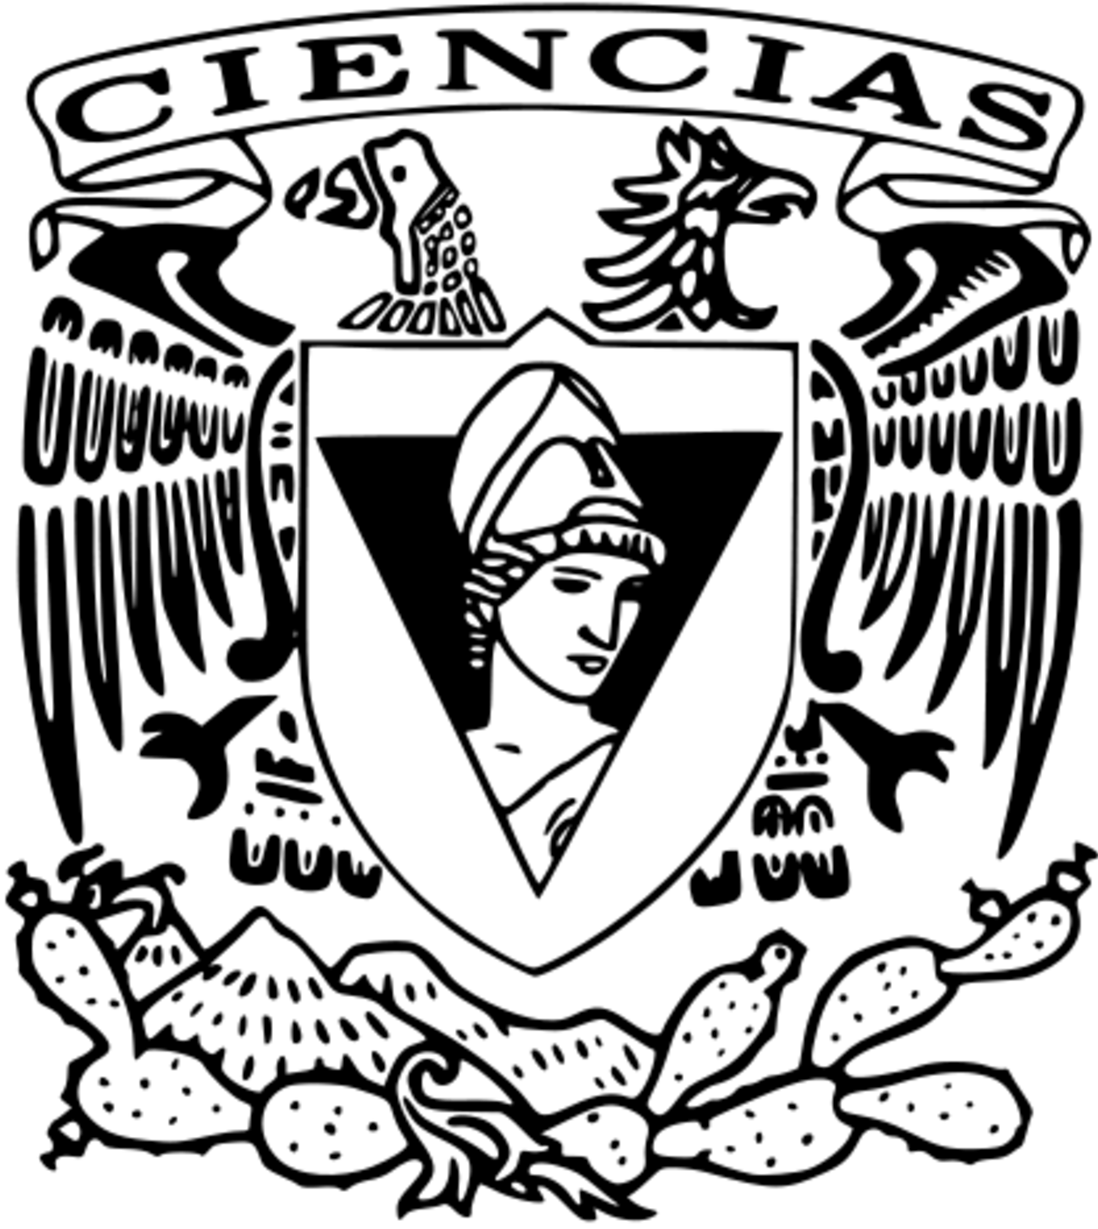
\includegraphics[height=3.4cm]{Logo_FC.png}
    	\end{center}
    \end{minipage}
\end{center}

\rule{17cm}{0.1mm}

\begingroup
  \let\clearpage\relax
  \let\cleardoublepage\relax

\begin{center}
{\Large\bfseries Resumen}
\end{center}

\begin{quote}
El problema a resolver es el desarrollo de un sistema de comunicación de mensajes usando el protocolo de red TCP; dicho problema se buscará atacar haciendo uso del método de desarrollo de la cascada, dicho método estará plasmado en este reporte (exceptuando el paso del mantenimiento); se abordará el análisis del problema para que con base en ello, podamos efectuar un diseño que nos pueda servir como guía para atacar el planeteamiento preestablecido, gracias a ello, podremos hacer uso de algún lenguaje de progrmación que se acople a nuestras necesidades para poder llevar a cabo la implementación de nuestro diseño. Cada una de las etapas previamente mencionadas podrán ser visibles en este reporte, para que, como resultado final, tengamos un resultado exitoso del sistema a desarrollar.
\end{quote}
  
  \chapter{Introducción al problema}

\noindent  Como primer proyecto de la materia de \textit{Modelado y Programación} se nos pide hacer el desarrollo de un sistema chat, el cual en esencia consiste en el intercambio de información entre las dos entidades involucradas en el protocolo de red TCP, dichas entidades son \textit{Cliente} y \textit{Servidor}.

\vspace{0.2cm}

\noindent  La importancia de realizar este primer poryecto es tener un primer acercamiento a lo que involucra el desarrollo de software, pues a diferencia de cursos pasados donde probablemente lo primero que se hacía era ir al teclado a generar código e ir improvisando durante el camino, en este curso justamente como su nombre indica, es demostrar la importancia que tiene tener un análisis del problema que se propone para poder generar un diseño independiente de las tecnologías que se pueden implementar para resolver el problema, pues de esa manera la etapa de la implementación resulta ser más limpia, y así,  poder realizar el proyecto de una manera optima; es por lo anterior, que se ve la importancia de este primer proyecto, para empezar a tener las base de buenas prácticas al momento de desarrollar software.

\vspace{0.2cm}

\noindent  Este proyecto de manera inherente presenta tanto dificultades como facilidades; iniciando con las dificultades, vemos que al inicio de este proyecto no cuento con varios de los conocimientos que se necesitan para poder dar una solución, conceptos como concurrencia, conexiones de red, programación teniendo como base un protocolo dado, uso de los objetos de tipo json, uso de interfaces gráficas (y muchos demás conceptos), esto es una dificultad pero a la vez es una oportunidad para poder ampliar la visión sobre el tipo de programas que puedo desarrollar, además de tener la necesidad de tener que aprender a manejar esos conceptos, y así agregar herramientas nuevas que en algún futuro me serán de gran utilidad; es por ello que si, el proyecto presenta un nivel avanzado por el manejo de nuevos conceptos y el poco tiempo que se tiene para manejarlos, pero sus facilidades y viendo luz en la oscuridad, es una nueva oportunidad para aprender.

\vspace{0.2 cm}

\noindent Sin embargo las dificultades previamente mencionadas, corresponden a tecnologías particulares, las cuales debemos pensar de una manera más abstracta, pues al momento de dar un análisis y diseño  a nuestro problema, estos deben ser pensados de manera general sin todavia estar pensando totalmente en todas las tecnologías que implemenetaremos, es por ello, que plasmar dicha parte del desarrollo es importante para poder dar un buen código, por esa razón es que se hace este reporte del proyecto, pues si bien, podemos decirnos a nosotros mismos que el análisis ya lo tengo en la cabeza, es importante poder plasmarlo, así como tambien es importante plasmar nuestro diseño, aunque esto se pueda escuchar tedioso, veremos que si hacemos una buena etapa de modelado, la parte de la implemenación resultará ser más sencilla (o eso es lo que se espera)

\vspace{0.2 cm}

\noindent Asi vemos que el desarrollo de la aplicación del chat, inmiscuye diversas problematicas que abordaremos a continuación

\vspace{0.2cm}




    \chapter{Análisis del problema}


\noindent Ya que definimos el problema a resolver, debemos enfocarnos en como atacar el problema. Siguiendo las recomendaciones sobre que aspectos debemos tener en cuenta antes de iniciar a programar, es necesario hacernos la pregunta ¿Es computable el problema planteado? Más alla de decir que "si" por el hecho de ser un proyecto para una materia de una carrera enfocada en las ciencias computacionales, diremos que si lo es, dando argumentos más sólidos. 

\vspace{0.5cm}

\noindent Podemos, de una manera abstracta, pensar a un chat como un sistema el cual se encarga de recibir información, procesar dicha información y mandar información. Además, revisando el protocolo ya dado, podemos ver que las operaciones establecidas en él (algunos ejemplos que podemos dar son  \textit{IDENTIFY, DISCONNECT, INVITE}) pueden modelarse mediante el uso de algortimos, por lo que al un chat ser la integración de aquellas operaciones, podemos decir que en efecto el problema que nos estan dando es computable.

\vspace{0.5cm}

\noindent Una vez que ya hemos concluído que el problema es computable, pasaremos a una etapa del análisis sumamente importante, que será aplicar la técnica \textit{"divide y vencerás"}, donde dividiremos nuestro problema en múltiples subproblemas a los cuáles buscaremos modelarles una solución.

\noindent Iremos usando un diseño de árbol para poder ver de una manera gráfica los problemas y subproblemas que iremos encontrando. Como raíz de nuestro árbol, tenemos nuestro problema principal el cuál es \textit{Aplicación Chat}

\vspace{0.5cm}
\begin{figure}[h]
\centering

\begin{tikzpicture}
\node[draw, rounded corners] {Aplicación Chat};
\end{tikzpicture}

\caption{Aplicación Chat}
\label{fig:aplicacion-chat}
\end{figure}

\vspace{0.5cm}

\noindent Nuestro chat, estará conformado por el intercambio de comunicación entre un \textit{servidor}, el cuál se encargará de manejar las instrucciones, que a su vez, serán enviadas por un usuario, o en otras palabras, un \textit{cliente}; por lo que añadimos a dichas entidades como subproblemas a resolver.

\begin{figure}[h]
\centering

\begin{tikzpicture}[
every node/.style={draw, rectangle, rounded corners}
]

\node (A) {Aplicación Chat};
\node (B) [below left=of A] {Servidor};
\node (C) [below right=of A] {Cliente};

\draw (A) -- (B);
\draw (A) -- (C);

\end{tikzpicture}

\caption{Estructura de la aplicación}
\label{fig:estructura-aplicacion}
\end{figure}

\vspace{0.5cm}

\noindent Sin embargo, como hemos mencionado "intercambio de información", vale la pena preguntarnos "¿Qué es la información mutua que ambas entidades estarán compartiendo?" La respuesta a esta pregunta la tenemos en el protocolo establecido, dado que es a través de este que definimos como tanto el cliente como el servidor intercambiaran información, esta es una capa que debe vivir simultanea a ambas entidades, pues ambas deben poder tener acceso a él.

\vspace{0.5cm}
\begin{figure}[h]
\centering

\begin{tikzpicture}[
every node/.style={draw, rectangle, rounded corners}
]

\node (A) {Aplicación Chat};
\node (C) [below=of A] {Protocolo};
\node (B) [below left=of C] {Servidor};
\node (D) [below right=of C] {Cliente};

\draw (A) -- (B);
\draw (A) -- (C);
\draw (A) -- (D);

\end{tikzpicture}

\caption{Estructura tomando en cuenta el protocolo}
\label{fig:protocolo-chat}
\end{figure}

\vspace{0.5cm}

\noindent Este análisis es la base para poder dar una idea sobre como es que se intercambiará la información entre ambas entidades, pero ahora hay que analizar cada una de ellas por separado, pues si bien todas estan dentro de un mismo sistema, cada una tiene sus propias maneras de comportarse.
\noindent De esa manera iniciemos, analizando que componentes serán ideales que pertenezcan a nuestro servidor:

\vspace{0.5cm}
\begin{figure}[H]
\centering

\begin{tikzpicture}[
every node/.style={draw, rectangle, rounded corners}
]

\node (A) {Servidor};

\end{tikzpicture}

\caption{Servidor}
\label{fig:servidor}
\end{figure}

\vspace{0.5cm}

\noindent El servidor es aquel que manejará a los clientes que querrán comunicarse, sin embargo para que eso sea posible deberemos hacer que el servidor sea capaz de recibir conexiones, escucharlas y responderles, esta descripción la podemos simplifcar a $Iniciar$ $Servidor$.

\vspace{0.2cm}

\noindent Una vez que nuestro servidor sea capaz de hacer dichas gestiones deberá ser capaz de poder identificar las conexiones, pues cada una es distinta a la otra. Vemos que dichas conexiones por como esta dado el protocolo, las podemos catalogar como \textit{Clientes} u \textit{Usuarios} , asi cada una de ellas  podemos verla como una $Conexion-Cliente$.

\vspace{0.2cm}

\noindent De manera analoga, como en el proyecto se nos están pidiendo salas, vemos que es lógico que las salas vivan el servidor, pues es este el que se encarga de hacer las gestiones en ellas, ya sea permitir crearlas, borrarlas y demas acciones que correspondan a las salas. Asi que esto lo podemos ver simplemente como $Salas$.

\vspace{0.2cm}

\noindent Estas entidades viven dentro del servidor, sin embargo aún nos falta alguna entidad que sea capaz de recibir la comunicación con el cliente, pero más alla de eso, que sea capaz de poder manejar los mensajes del protocolo, a este ente le llamaremos $Manejar$ $Protocolo$

\vspace{0.2cm}

\noindent Por lo tanto nuestro árbol del servidor se ve de la siguiente manera: 


\vspace{0.5cm}
\begin{figure}[H]
\centering

\begin{tikzpicture}[
    every node/.style={draw, rectangle, rounded corners},
    node distance=2cm
]

\node (A) {Servidor};

\node (B) [below=2cm of A, xshift=-4.5cm] {Conexion-Cliente};
\node (C) [below=2cm of A, xshift=-1.5cm] {Iniciar-Servidor};
\node (D) [below=2cm of A, xshift=1.5cm] {Salas};
\node (E) [below=2cm of A, xshift=4.5cm] {Manejar Protocolo};

\draw (A) -- (B);
\draw (A) -- (C);
\draw (A) -- (D);
\draw (A) -- (E);

\end{tikzpicture}

\caption{Componentes principales del servidor}
\label{fig:componentes-servidor}
\end{figure}

\vspace{0.5cm}

\vspace{0.5cm}

\noindent Ahora analizaremos que componentes serián los ideales que pertenezcan a nuestro cliente:

\vspace{0.5cm}
\begin{figure}[H]
\centering

\begin{tikzpicture}[
every node/.style={draw, rectangle, rounded corners}
]

\node (A) {cliente};

\end{tikzpicture}

\caption{Cliente}
\label{fig:cliente}
\end{figure}

\vspace{0.5cm}

\noindent El cliente es aquel ente que se conectará a nuestro servidor, pues este recibirá comunicación mutua del mismo, para ello denotaremos a un ente que se encargue de dichas acciones como $Iniciar$ $Cliente$.

\vspace{0.2cm}

\noindent De la misma manera en que en el Servidor, necesitamos una entidad que sea capaz de recibir la comunicación mutua con el servidor, pero esta comunicación no es arbitraria sino que esta dada por el protocolo, por tanto aquí tambien es necesario tener una entidad llamada $Manejar$ $Protocolo$

\noindent Una entidad que es distintiva del cliente a comparación del servidor, es que en nuestro cliente debemos ser capaces de mostrar la información que estamos recibiendo del servidor, por tanto podemos pensar en una entidad abstracta (abstracta en la definción de la palabra, no de un lenguaje de programación) llamada \textit{Mostrar-Informacion}

\vspace{0.2cm}

\noindent Por lo tanto nuestro árbol del servidor se ve de la siguiente manera: 

\vspace{0.5cm}
\begin{figure}[H]
\centering

\begin{tikzpicture}[
    every node/.style={draw, rectangle, rounded corners},
    node distance=2cm
]

\node (A) {Cliente};

\node (B) [below left=of A] {Iniciar Cliente};
\node (C) [below=of A] {Manejar Protocolo};
\node (D) [below right=of A] {Mostrar Informacion};

\draw (A) -- (B);
\draw (A) -- (C);
\draw (A) -- (D);

\end{tikzpicture}

\caption{Componentes principales del cliente}
\label{fig:componentes-cliente}
\end{figure}

\vspace{0.5cm}

\noindent Del árbol del cliente, podemos visualizar un problema, estamos dividiendo y venciendo, sin embargo el ente de \textit{Mostrar-Infomracion} es un subproblema que nos puede llevar a más subproblemas, pues pensando en como es un chat, este tiene diversas maneras de presentar la información, pues no es lo mismo recibir mensajes en una Sala general, que en una privada, como tampoco es lo mismo escribir a más de una persona como escribir un mensaje a alguien en partícular, por lo tanto el nodo al que estamos haciendo referencia, puede tener otros nodos, los cuales llamaremos \textit{Chat-General}  , \textit{Chat-Privado} y \textit{Chat-En-Sala}. Asi nos quedaria el árbol del nodo \textit{Mostrar-Informacion}:

\vspace{0.5cm} 

\begin{figure}[H]
\centering

\begin{tikzpicture}[
    every node/.style={draw, rectangle, rounded corners},
    node distance=2cm
]

\node (A) {Mostrar-Información};

\node (B) [below left=of A] {Chat-General};
\node (C) [below=of A] {Chat-Privado};
\node (D) [below right=of A] {Chat-En-Sala};

\draw (A) -- (B);
\draw (A) -- (C);
\draw (A) -- (D);

\end{tikzpicture}

\caption{Opciones de visualización de información}
\label{fig:mostrar-informacion}
\end{figure}

\noindent Tras revisar los problemas que deberemos afrontar para la realización del proyecto (así como de sus subproblemas), podemos destacar lo siguiente:
Durante el desarrollo de los árboles hemos estado haciendo referencia a la palabra ``ente'' (u ``entidad''), esto debido a que sabemos que hay ``algo'' que queremos que tenga una cierta responsabilidad en nuestro sistema, pues resulta coherente que no podemos englobar todas las acciones que queremos que haga el chat en una sola; dicho ``ente'' aun no sabemos exactamente como se comportara, pero si sabemos que resultado deseamos obtener; por tanto podemos decir que es un ``Objeto'' con propiedades y responsabilidades unicas, asi que resulta aún mas coherente que una manera de abordar este proyecto es utilizando el paradigma orientado a objetos, pues vemos que tras realizar el análisis, el proyecto practicamente nos esta gritando ``!!!Modela esto como un objeto!!!''.

\vspace{0.2cm}
\noindent Asi que, una vez que hemos analizado el problema, viendo que casos debemos atacar y concluyendo que la mejor manera de abordarlo es mediante Orientación a Objetos pasaremos a la siguiente etapa del método cascada que es el \textit{DISEÑO} 

\chapter{Diseño de la solución al problema}

\noindent Hemos avanzado a la siguiente parte de nuestro desarrollo, el diseño asi que ahora vale la pena preguntarnos ¿Qué patrones de diseño es conveniente utilizar para el desarrollo de la aplicación?. Aqui la respuesta que hemos elegido (además de que fue petición por parte del profesor) es utilizar el patrón de diseño \textit{MVC} (Modelo,Vista,Controlador).

\vspace{0.2cm}

\noindent Este patrón de diseño se ajusta muy bien a las necesidades que tenemos, pues como describimos en nuestro análisis, algo que si bien no es imposición pero si nos puede facilitar el desarrollo, es tener separadas las responsabilidades que tendrán los objetos involucrados en nuestro sistema; MVC justamente nos ayuda a este problema, pues es una manera muy ``visible'' de identificar que responsabilidades serán parte, ya sea de nuestra vista, nuestro modelo o nuestro controlador.

 \vspace{0.2cm}

 \noindent Justamente como hemos decicido trabajar en separar lo más posible las responsabilidaes, es que una decisión de diseño que tomaremos es tener dos programas distintos, es decir el programa del \textit{Cliente} y el programa del \textit{Servidor}; bien pudimos haber tomado la deicisión de tener ambos en un mismo programa, y sobre ello trabajar con MVC, pero no considero que sea una decisión favorable, pues como ejemplo en un mismo modelo vivirian nuestra de manera de conectar al servidor, la lógica de los cuartos, la lógica de hacer la conexión del cliente; que si bien vemos que aún asi se mantiene el diseño del modelo en MVC, desde que lo vemos escrito no suena coherente que la manera en que conectamos el cliente al servidor viva en la misma capa que la logica de las salas.

 \vspace{0.2cm}
 
 \noindent Por lo anterior se ha decidido que el Cliente tenga su propio diseño de MVC, asi como el servidor tenga su propio diseño de MVC, pues de esa manera las responsabilidades de cada uno se reparten de una mejor manera.

 \vspace{0.2cm}

 \begin{figure}[h]
    \centering
    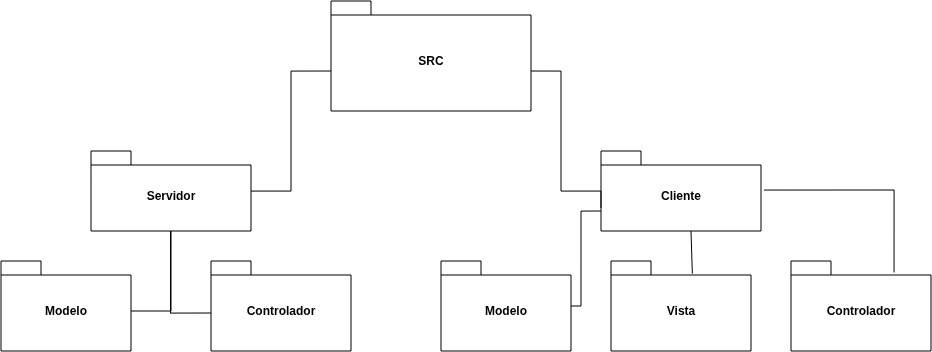
\includegraphics[width=0.8\textwidth]{aaaa.jpg}
    \caption{Diagrama de las capas del sistema.}
    \label{fig:capas}
\end{figure}

\noindent Vemos que en la Figura~\ref{fig:capas} servidor no tiene la capa de Vista, esto es coherente pues el servidor solo debe de existir como un ente que sea capaz de gestionar las conexiones de los clientes, en cambio vemos que en el cliente si tenemos la capa de vista, pues aqui si debemos de mostrar la información correspondiente al chat.

\vspace{0.2cm}

Vemos que en nuestra Figura~\ref{fig:capas} no incluimos la capa del \textit{Protocolo}, esto porque en dicha capa no aplicaremos MVC, pues dicha capa solo la estaremos usando para almacenar los mensajes que estan involucrados en el protocolo, por ello el diagrama de como estará la capa de \textit{Protocolo} la podemos ver de la siguiente manera:

 \begin{figure}[h]
    \centering
    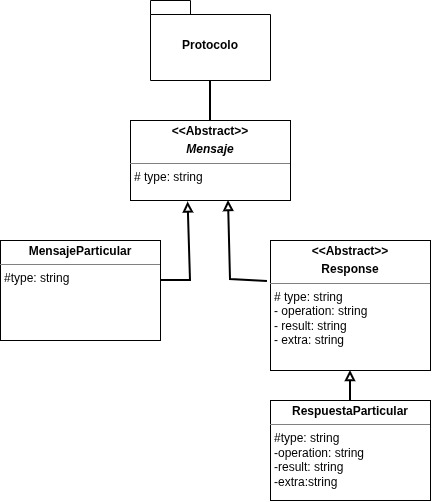
\includegraphics[width=0.5\textwidth]{protocolo.jpg}
    \caption{Diagrama de la capa del protocolo.}
    \label{fig:protocolo}
\end{figure}

\noindent En esta decisión de diseño vemos que los mensajes los vamos a representar como objetos, pero solo con atributos que es donde guardaremos la información necesaria de cada mensaje; en la Figura~\ref{fig:protocolo} vemos que todos los tipos de mensaje heredarán de la clase \textit{Mensaje}, pues al revisar el protocolo vemos que cada uno de los mensajes tiene como atributo un \textit{type}; de aquí vemos que la clase de \textit{MensajeParticular} representará los disitintos tipos de mensaje que deberemos manejar, no quiere decir que solo vaya a haber una clase llamada MensajeParticular, sino que solo es la representación de todos los demas mensajes que pueden llegar a habe.

\vspace{0.2cm}

\noindent Del lado contrario vemos que heredamos la clase \textit{Response}, esto es debido a que muchos mensajes distintos actuan como respuesta, y su \textit{type} siempre esta asociado con \textit{RESPONSE}, por ello de esta clase hereda otra llamada \textit{RespuestaParticular} que podemos describir de la misma manera que describimos \textit{MensajeParticular}, pues solamente es la representación de los distintos tipos de respuesta que hay en el protocolo.

\vspace{0.2cm}

\noindent Siguiendo con nuestro diseño, ahora plantearemos el diseño que vamos a usar en el Servidor; previamente en nuestro análisis obtuvimos que los objetos que nos ayudarán a resolver los problemas que presenta el servidor son: \textit{Conexion-Cliente, Iniciar-Servidor, Salas, Manejar-Protocolo.}
Describiremos de mejor manera como es que cada uno de ellos nos ayuda a llegar al resultado de tener un servidor funcional:

\vspace{0.2cm}

    \begin{itemize}
        \item[-] \textbf{Conexion-Cliente}\\
        \noindent Conexion-Cliente representará la conexión que tiene el cliente con el servidor, suena redundante, pero en particular este objeto se refiere a que cada que el cliente se conecte con el servidor, se le asigne una instancia de Conexion-Cliente, que nos servirá para identificar a ese cliente (usuario) en especifíco en la aplicación del chat; por lo anterior es que Conexion-Cliente puede tener como atributos: \textit{username, status, socket} con el cual se intercambiará la información. Mientras que los metodos que podemos pensar son: 
                    \begin{itemize}
                \item[-] {\textit{RecibirMensajes:}} Este método nos servirá para poder recibir los mensajes que vendran del cliente
                \item[-] {\textit{EnviarMensaje:}} Este método nos serviŕa para poder enviar un mensaje al cliente, este nos servira para poder enviar mensaje de tipo \textit{RESPONSE} requeridos por el protocolo.
            \end{itemize}
        \item[-] \textbf{Iniciar-Servidor}\\
        \noindent Iniciar-Servidor será aquel objeto que ponga nuestro servidor en la red, para que de esa manera los clientes puedan conectarse, pensando de esa manera vemos que los atributos que puede tener el objeto son: \textit{puerto, socket}. (que dicho socket será de escucha).
        Pensando en que acciones ejecutaŕa el objeto podemos pensar en los siguientes metodos:
            \begin{itemize}
                \item[-] {\textit{Iniciar:}} Iniciamos el servidor para poder recibir clientes.
                \item[-] {\textit{AceptarClientes:}} Una vez que inciamos el servidor, permitimos que clientes se conecten a nuestro servidor.
            \end{itemize}
            
        \item[-] \textbf{Sala}\\
        \noindent Este objeto funcionará de manera general como una estructura de datos en la cual podemos almacenar conexiones de clientes, esta estructura no tendria comunicación directa con el cliente, pues solo nos servira para guardar sus conexiones, por ello podemos pensar en atributos como: 
        nombre del cuarto, lista de invitados y lista de usuarios (esos dos ultimos atributos es debido a que en el protocolo se nos dice que una conexion puede tener los siguientes estados (referente a las salas): fue invitado a un cuarto o esta en un cuarto). Los metodos que nos permitiran manejar las acciones de la sala son:

             \begin{itemize}
                \item[-] {\textit{AgregarUsuario:}} Con este método podremos agregar un usuario al cuarto.
                \item[-] {\textit{EliminarUsuario:}} Con este método podremos eliminar un usuario del cuarto.
                \item[-] {\textit{Invitar:}} Con este método podremos mandar una invitación a un usuario.
                \item[-] {\textit{EliminarInvitado:}} Con este método podremos eliminar invitado de la lista de invitados (esto nos sirve pues si el usuario acepta la invitación pasa a la lista de usuarios, y deja la lista de invitados)
                 \item[-] {\textit{Vacio:}} Con este método podremos determinar si un cuarto se encuentra vacio, este nos servirá en particular pues el protocolo nos dice que un cuarto vacio debe ser eliminado, asi que saber si esta o no vacio es de gran utilidad.
                
            \end{itemize}
            
        \item[-] \textbf{Manejar-Protocolo}\\
        \noindent Como describimos en nuestro análisis estamos pensando que este objeto sea el encargado de recibir la comunicación con el cliente siguiendo el protocolo, es decir funcionará como nuestro puente entre ambas conexiones, por ello podemos pensar en atributos asociados como: \textit{Servidor, Lista de Clientes, Lista de salas.}
        Los metodos que podemos pensar para este objeto son los siguientes:
            \begin{itemize}
                \item[-] {\textit{NuevaConexion:}} Con este método asociar la conexion que nos llega, agregando la conexión a nuestra lista de clientes.
            \end{itemize}
        \noindent Ahora bien aquí vale la pena deternenos, estamos diciendo que el objeto de \textit{Manejar Protocolo} es quiem hara el manejo de la comunicación con el cliente, como dicha comunicación esta dada por el protocolo, y ademas por el paso anterior decidimos que la capa de protocolo maneja la comunicación con clases de \textit{Mensaje}, entonces vemos que \textit{Manejar Protocolo} debe ser capaz poder manejar dichos tipos de \textit{Mensaje}, por lo tanto podemos definir la siguiente operación:
            \begin{itemize}
                \item[-] {\textit{Tipo-De-Mensaje:}} Este metodo nos permite hacer el manejo del mensaje que recibamos por parte de la comuncación que tenemos con el cliente
            \end{itemize}
        Dicho método dependerá de si recibimos ``IDENTIFY'', ``TEXT'', ``USERS'' y demas mensajes que estan definidos en el protocolo.
        
    \end{itemize}

\noindent De los anteriores objetos observamos que si seguimos nuestro patrón de diseño MVC, podemos clasificar cada Objeto de esta manera:
            \begin{itemize}
                \item[-] {Modelo:} Iniciar-Servidor, Sala, Conexion-Cliente
                \item[-] {Controlador:} Manejar-Protocolo
            \end{itemize}

\noindent Por lo tanto podemos dar el siguiente diagrama:

 \begin{figure}[H]
    \centering
    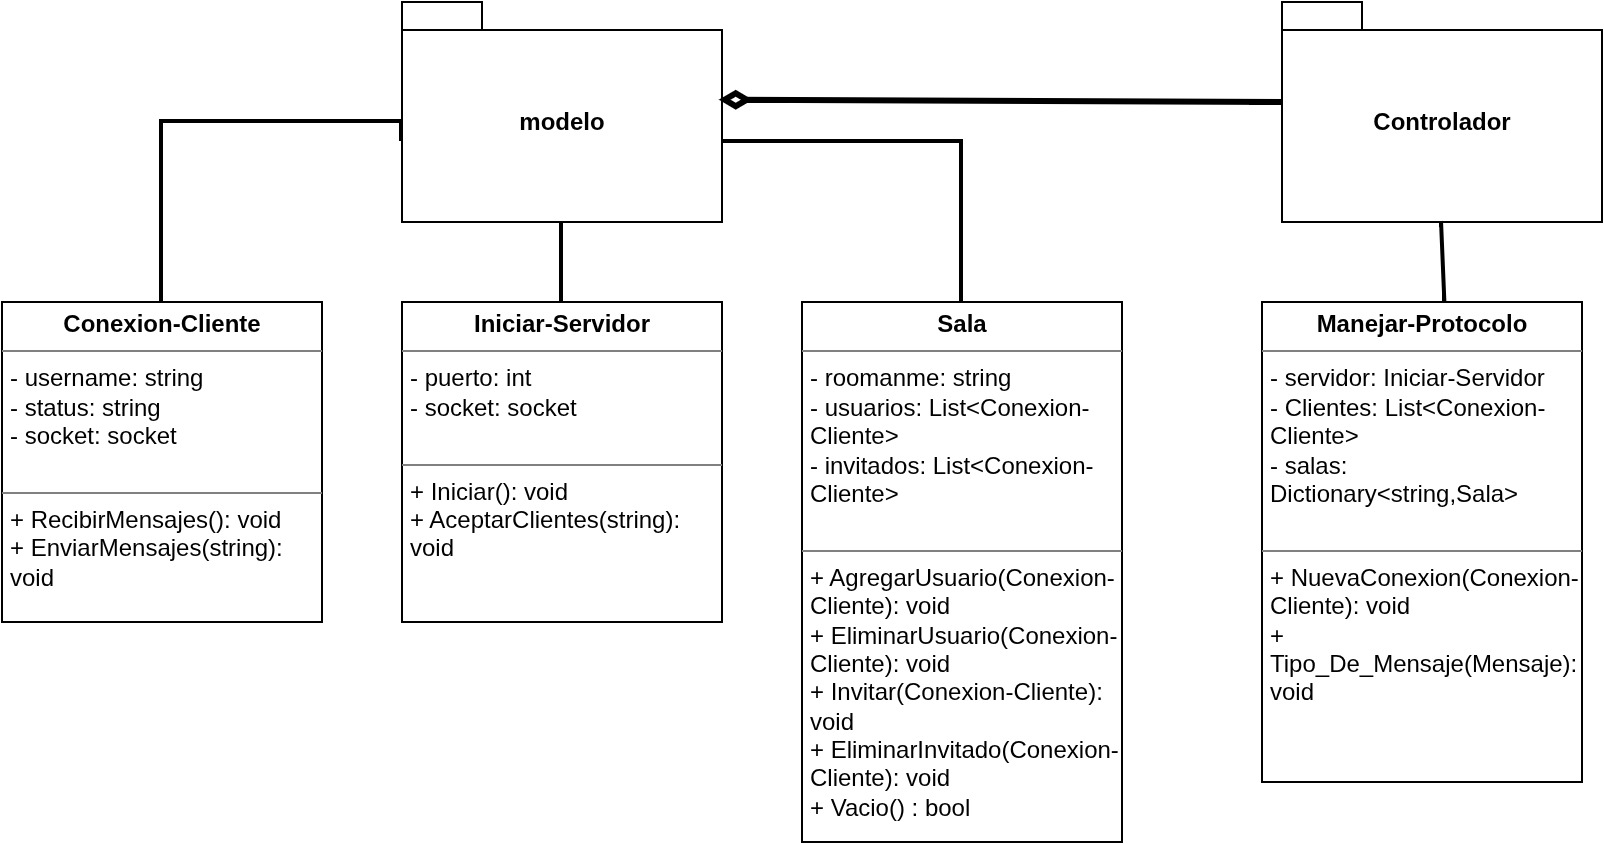
\includegraphics[width=0.9\textwidth]{ServidorDiagrama.jpg}
    \caption{Diagrama del servidor.}
    \label{fig:servidorDiagrama}
\end{figure}

\vspace{0.5cm}
\noindent Una vez que ya hemos diseñado una solución a nuestro servidor, vamos a pasar con el cliente.
\noindent En el lado del cliente durante nuestro análisis logramos identificar a objetos u entes que nos pueden ayudar a modelar una solución para poder tener un cliente funcional, dichos entes fueron: \textit{Iniciar Cliente, Manejar Protocolo, Mostrar Informacion}.
Por tanto vamos a describir de mejor manera a dichos objetos para poder ver como es que participarán en nuestro diseño de la solución.
    \begin{itemize}

        \item[-] \textbf{Iniciar Cliente}\\
        \noindent Este objeto nos servirá como lo describimos en nuestro análisis para poder hacer hacer la comunicación mutua con el servidor, viendolo de esta manera podemos dar los siguientes atributos: \textit{Socket}, que se encargará de poder hacer la conexión con el servidor.
        Así ahora, podemos pensar en los metodos que implementa nuestro objeto:

             \begin{itemize}
                \item[-] {\textit{Conectar:}} Con este método podremos realizar la conexión con el servidor.
                \item[-] {\textit{EnviarMensaje:}} Este método nos permitira enviar datos a nuestro servidor, y dado que estamos usando sockets, lo podremos hacer usando el Write() del mismo.
                \item[-] {\textit{RecibirMensaje:}} Al utilizar este método podremos recibir los datos que el servidor esta mandando a nuestro cliente, como estamos trabajando con sockets podremos hacer esta función usando el Read() asociado al socket.
            \end{itemize}

        \item[-] \textbf{Manejar Protocolo}\\
        \noindent Este objeto tiene una finalidad análoga al Manejar Protocolo del servidor, pues en esencia se encarga de procesar la comunicación que hay entre el servidor y el cliente, y como la comunicación viene dada por el protocolo, ese método tiene como finalidad manejar los mensajes del protocolo, así entonces podemos definir los atributos: \textit{Iniciar Cliente}, pues asi tenemos una instancia \textit{Iniciar Cliente} que mediante sus metodos de Recibir y Enviar Mensaje podra procesar los mensajes enviados por el servidor, y mandar mensajes al mismo.
        Ahora, pensamos en la definición de nuestros metodos
            \begin{itemize}
                \item[-] {\textit{Tipo-De-Mensaje:}} Este método nos permite hacer el manejo del mensaje que enviemos por parte de la comuncación que tenemos con el cliente
                \item[-] {\textit{MensajeRecibido:}} Este método nos permite hacer el manejo del mensaje que recibimos por parte de la comuncación que tenemos con el cliente
            \end{itemize}
                        \noindent Aquí vemos que con diferencia del servidor, el método \textit{Tipo-De-Mensaje} procesará el tipo de mensaje que nosotros mandemos hacia el servidor, esto es ya que los usuarios interactuarán en la aplicación a través del cliente, por ello debemos tener una manera de captar la acción que hacer el usuario para mandarla al servidor.
            \end{itemize}
            
        \vspace{0.2cm}
        
        \noindent Aquí detenemos un poco el diseño de la solución pues el siguiente problema que debemos afrontar es el de \textit{Mostrar-Información}. Durante nuestro análisis logramos identificar que en el cliente si debe haber una vista incorporada de MVC. La decisión de diseño que hemos tomado es que la vista será implementada por una interfaz gráfica. Esta es una decisión arriesgada dado que nunca he realizado una interfaz gŕafica, sin embargo en mi opinión un chat implementado en terminal queda muy limitado para la experiencia del usuario, pues es más intuitivo pensar en una interfaz gráfica y que dado que se presiona un botón se mande a llamar dicha acción; por lo anterior es que los sub-problemas que vienen con \textit{Mostrar-Informacion}, no son precisamente objetos, sino pestañas que queremos tener en nuestra interfaz gráfica.
                \vspace{0.2cm}
                
        \noindent Así tambien resaltamos que \textit{Mostrar-Información} tampoco es un objeto perse, sino una manera de representar que es en esa parte del cliente donde estará implementada la lógica de nuestra interfaz, es decir, dejando el lado abstracto que teniamos en el análisis, \textit{Mostrar-Informacion} sería la capa de Vista del patrón MVC.

        \vspace{0.2cm}

        \noindent Entonces dado que ya hemos descrito las partes que conforman a nuestro cliente, podemos asociar cada una de ellas las capas de MVC, quedando de la siguiente forma:
            \begin{itemize}
                \item[-] {Modelo:} Iniciar-Cliente
                \item[-] {Controlador:} Manejar-Protocolo
                \item[-] {Vista:} Mostrar-Información
            \end{itemize}
        \vspace{0.2cm}

        \noindent Ahora nuestro diagrama del cliente se ve de la siguiente forma:

\begin{figure}[H]
    \centering
    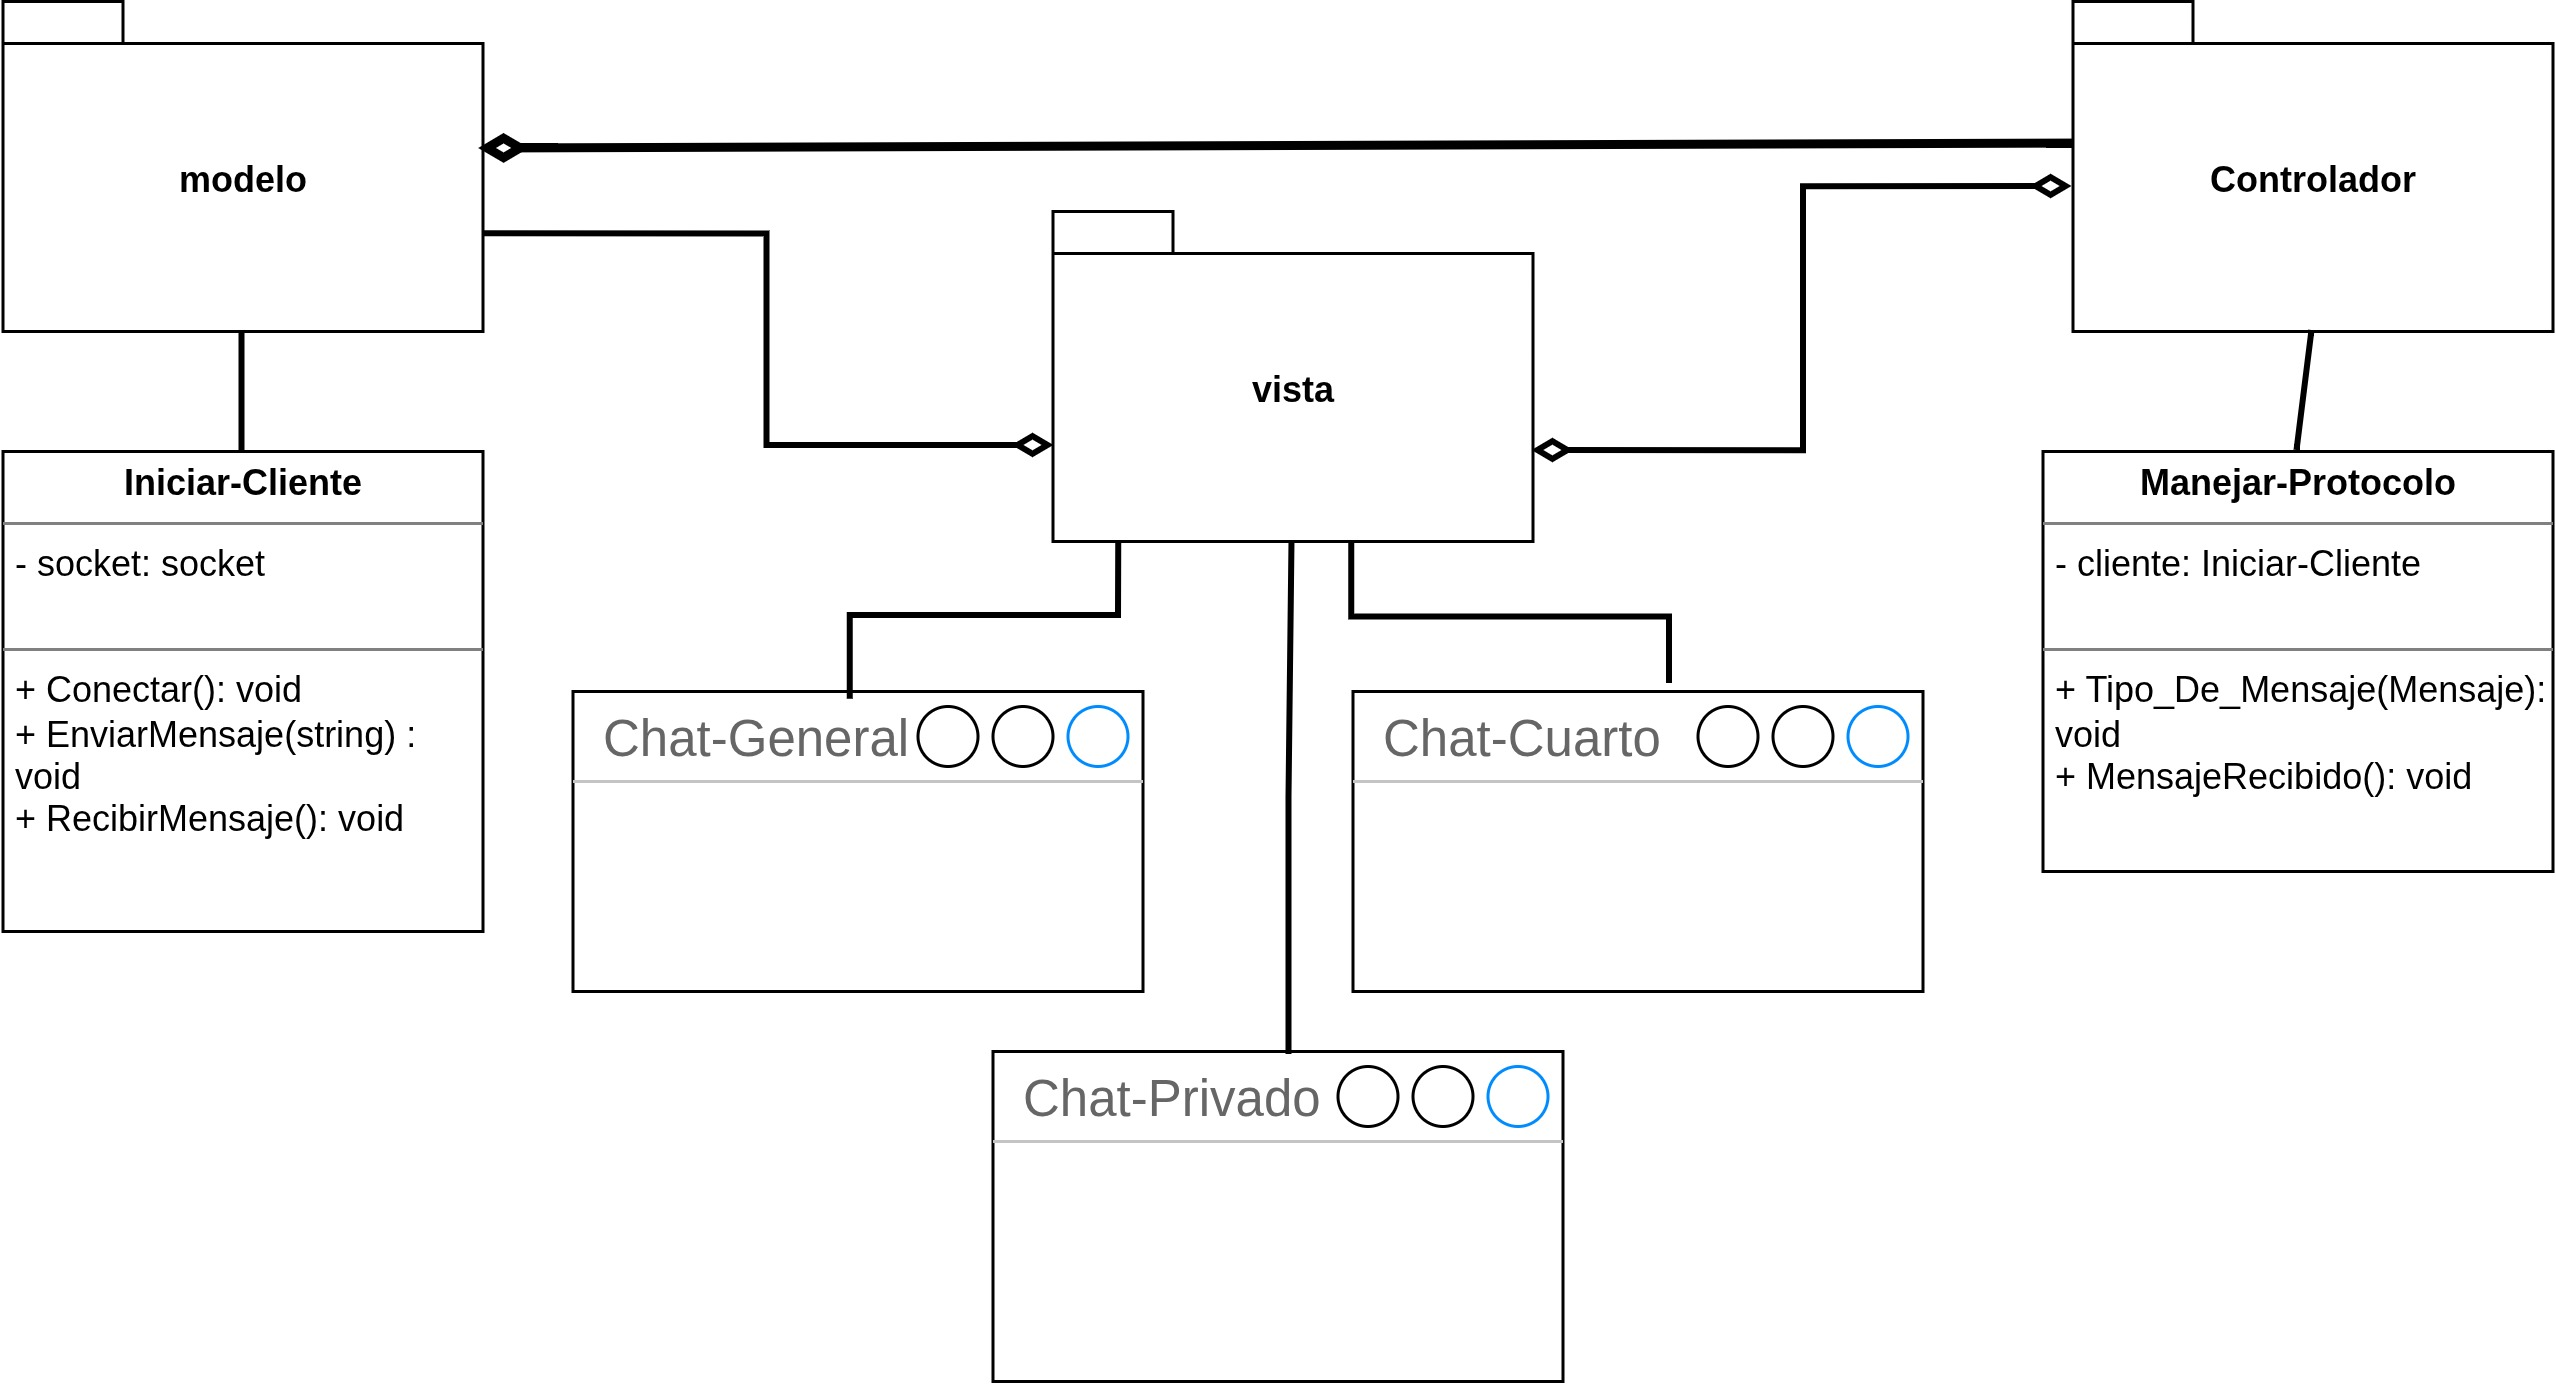
\includegraphics[width=0.9\textwidth]{ClienteDiagrama.jpg}
    \caption{Diagrama del cliente}
    \label{fig:diagramaCliente}
\end{figure}

\vspace{0.5cm}
    \noindent Hemos diseñado la manera en que abordaremos el problema del chat, el diseño es independiente del lenguaje de programación sin embargo utilizar un lenguaje de programación cuyo paradigma este orientado a objetos resulta una mejor decisión de diseño.

    \vspace{0.2cm}

    \noindent Se nos dió la opción de trabajar el proyecto usando C en el servidor, este opción fue considerada, sin embargo al C no estar inherentemente orientado a objetos ciertas operaciones de nuestro diseño podrían ser más dificles de implementar, entonces por esa razón trabajar el servidor en C queda descartado.

    \vspace{0.2cm}

    \noindent Por lo anterior es que se decidió que tanto el servidor como el cliente estarán escritos en el lenguaje C\#, pero ¿por qué esta decisión?, esta decisión se tomó debido a que durante mi experiencia como estudiante de CC, solo he trabajado en el lenguaje de Java (que esta prohibido), y tras una investigación en internet, C\# es un lenguaje parecido a Java, y dado que el tiempo es reducido acostumbrarme a una sintaxis distinta podría ser ponerme un pie a mi mismo, asi que por practicidad se eligió como lenguaje principal C\#.

    \chapter{Implementación del diseño}

    \noindent Después de tener nuestro diseño del cual rescatamos como vamos a manejar tanto al cliente, servidor, los mensajes del protocolo, el paradigma que usaremos, así como el lenguaje de programación que vamos a utilizar, damos pie a la implementación del diseño, donde vamos a hablar de las tecnologías que utilizamos.

    \noindent Primero es necesario hablar de una refactorización que hicimos en los nombres de las clases que describimos en nuestro diseño, pues al momento de sentarme a programar me di cuenta que probablemente los nombres no representaban de manera correcta su función, es por ello que tuvimos los siguientes cambios:

    \vspace{0.2cm}

    Del lado del servidor:

    \begin{itemize}
        \item[-] Conexion-Cliente → ConexionCliente
        \item [-] Iniciar-Servidor →Servidor
        \item [-] Iniciar-Servidor → Servidor
        \item [-] Sala → Cuarto (se me hizo más comodo usar el nombre de cuarto para representar las salas)
        \item [-] Manejar-Protocolo → ServidorControlador (pues en el diseño vimos que está clase es el controlador de nuestro modelo MVC)
    \end{itemize}

    Del lado del cliente:

    \begin{itemize}
        \item[-] Iniciar-Cliente → ConexionServidor (pues es la conexión que hay con el servidor)
        \item [-] Iniciar-Servidor → Servidor
        \item [-] Manejar-Protocolo → ClienteControlador (pues en el diseño vimos que está clase es el controlador de nuestro modelo MVC)
        \item [-] Chat-General → VentanaChat
        \item [-] Chat-Privado → ChatPrivado
        \item [-] Chat-Privado → CuartoPrivado

    \end{itemize}

    \vspace{0.2cm}

        \noindent \textbf{Implementación de la conexion Cliente-Servidor}

    \noindent Después, vemos que la base del proyecto es poder tener comuncación de red entre el servidor y el cliente, por lo general y en bajo nivel podemos utilizar sockets junto a sus operaciones asociadas como \textit{bind(), listen(), write()} y demás; pero investigando que cualidades y facilidades que nos da nuestro lenguaje C\# , encontré dos clases que simplifican de manera muy grande tener que trabajar diectamente con sockets, dichas clases son \textit{TcpCliente y TcpListener},  de las cuales vamos a hablar:
    \begin{itemize}
        \item[-] {TcpListener:} TcpListener nos ayuda a supervisar un puerto TCP que va a buscar las soliciudaes entrantes y luego crear objeto TcpClient que administre la conexión del  cliente. Vemos que funciona como el socket que se encargará de admnistrar el servidor, es por ello que este se utiliza en la misma clase \textit{servidor}, con los métodos \textit{Start(), AcceptTcpClientAsync()} así como el construtor de la clase TcpListener, que es aquí donde iniciamos el servidor con una dirección IP y un puerto; usando las operaciones anteriores es que podemos tener nuestro servidor funcional.
        \item[-] {TcpClient:} Esta clase la usamos para crear una conexión de cliente a un host remoto, aquí se abstraen los detalles para que creemos un Sockett con el fin de solicitar y recibir datos mediante TCP, es decir en palabras más sencillas, es el socket asociado a nuestro cliente.

        Por lo anterior es que TcpClient, lo llamamos tanto en el servidor como en el cliente, esto pues en nuestra clase \textit{ConexionCliente} se usa como el parametro para construir dicha clase, pues dicha clase representa los comportamientos que queremos que tengan nuestra conexiones una vez que llegan al servidor; sin embargo, tambien la usamos en nuestro Cliente, ya que en la clase \textit{ConexionServidor} es que lo usamos para conectarnos usando el metodo Conectar() al asociar nuestro objeto TCPclient con una dirección IP y puerto  (que son los mismos de nuestro TcpListener).
    \end{itemize}

    \noindent Además cabe señalar que tanto en el cliente como en el servidor, junto a TcpCliente y TcpListener conviven junto a la clase \textit{NetWorkStream} la cual nos proporciona un flujo de datos (stream) para enviar y recibir infomación, es por ello que esta clase la usamos en nuestros métodos de RecibirMensajes() y EnviarMensaje() pues con sus métodos como ReadAsync() y WriteAsync() es que podemos hacer el flujo de mensajes.

    \vspace{0.3cm}

    \noindent \textbf{Uso de eventos y programación asíncrona}
    
    \noindent Otro de los recursos que nos proporciono nuestro lengauje de programación fue el uso de Eventos, esta herramienta fue nueva de trabajar para mi, pues antes de saber como llevar mi diseño a su implementación no sabia que existian, sin embargo, estos fueron de mucha utilidad para el programa; vemos que los eventos nos permiten notificar a otros objetos cuando ocurre una acción, esto lo usamos usando las bases que definen al evento, que son \textit{publisher, suscriber y delegate}
    
    \vspace{0.2 cm}

    \noindent Vemos que estas herramientas nos son utiles pues en el chat no estamos esperando un flujo secuencial, pues esto podría bloquear al programa cuando otro usuario haga alguna otra acción como escribrir, por eso al usar eventos, vemos que cada suceso se atenderá al momento sin bloquear a los demás clientes.


    \vspace{0.2 cm}
    
    \noindent Los eventos los usamos en nuestro servidor de la siguiente forma:
    Declaramos nuestro evento \textit{nuevaConexion} e invocamos cada vez que se acepte un cliete de manera asincrona (todo esto sucede en la clase \textit{servidor}), seguido de ello en la clase \textit{ServidorControlador} hacemos la suscripción del evento al método NuevaConexion. de esa manera cada que llegue una conexión y la aceptemos podremos manejarla desde ServidorControlador; algo casi analógo hacemos con el evento mensajeRecibido en la clase \textit{ConexionCliente} pues este se va a disparar cuando se invoque al metodo de RecibirMensaje(), y haremos la suscripción de dicho evento en el método de NuevaConexion().

    \noindent(El uso de eventos en el cliente se usa de manera analóga como se uso el evento MensajeRecibido en nuestro servidor)

    \vspace{0.2cm}

    \noindent Como siguiente punto importante a mencionar en nuestra implementación, es que al revisar el código vemos que no se están viendo explicitamente el uso de hilos de ejecución, pues debido (nuevamente) a las facilidades que nos proporciona C\#, vemos que trabajamos con programación asincrona, usando metodos \textit{async} y \textit{Task}; esto lo maneje de esta forma pues al usar \textit{Task} (que representa una operación que ya inicio pero aún no termina) podemos hacer que un método se supenda sin tener que bloquear el hilo, esto lo hacemos usando \textit{await} , así en cuando se termine la tarea, el método sigue donde quedo esperando; lo anterior me parece que funciona bien pues en el chat practicamente lo único que hacemos son operaciones de entrada y salida, y hacer que estas operaciones no se mezclen entre sí fue manejable usando la programación asincrona que nos dio C\#.

     \vspace{0.3cm}

            \noindent \textbf{Interfaz gráfica} 
    

     \noindent En la implementación del diseño, vemos que en la vista simplemente definimos que tanto \textit{Chat-General, Chat-Privado y Chat-Cuarto} serían pestañas de la interfaz que ibamos a integrar al sistema, al mometno de diseñar la solución eso lo podiamos dejar de manera abstracta, pero al momento de hacer la implementación ya era necesario encontrar una manera integrar una interfaz gráfica a nuestro proyecto, es por ello que se utilizó el framework \textit{Avalonia}; investigando encontré que una manera de realizar interfaces gráficas en C\# era justamente con el framework mencionado, si bien habia otras opciones como \textit{WinForms}, se decidió usar Avalonia por sus comptabilidad en sistemas linux. El usar avalonia fue algo completamente nuevo pues nunca había trabajado con algo parecido, es por ello que la interfaz gráfica, si bien es muy mejorable cumple con lo más básico que deberia ser capaz de hacer, esto pues el uso básico de avalonia no es muy dificl de entender, pues por cada \textit{axaml} que generemos, deberemos tambien generar su \textit{axaml.cs} que será la manera en que podamos interactuar; si vemos, nuestra interfaz gráfica solo esta conformada por \textit{TextBlock, TextBox, TabItem }y \textit{Button}, que al interactuar con ellas (sobre todo con el Botton) estaremos enviando los mensajes en el formato que pide el protocolo al servidor, y el servidor al responder, los métodos de la interfaz sabrán que mostrar al usuario según el tipo de \textit{RESPONSE} recibido.

        \vspace{0.3cm}

        \noindent \textbf{Sistema de construcción y documentación}
    
     \noindent Como siguiente punto a destacar fue la decisión de usar \textit{MakeFile} para nuestro sistema de construccion, si bien al parecer el entorno .NET ya trae incorporados métodos para el sitsema de construcción por medio de dotnet, el usar MakeFile se me hizo más comodo pues al simplemente colocar ``Make Accion'' se ejecuta la acción deseada, por ello el sistema se construye usando \textit{MakeFile}

     \noindent Para hacer generación de la documentación se utlizó DocFX, esto pues al momento de buscar de que maneras podia generar la documentación me salió como opción, siendo sinceros al ser de las primeras opciones que conocí y al ver que podia generar un sitio html para poder ver la documentación de manera similar a como lo hace javaDoc en Java, pues fue una buena decisión para mi; sin embargo, hay un ``problema'', pues al parecer para generar dicho sitiio, DocFx genera archivos JavaScript lo que hace que en el repositorio de Github marque que en los lenguajes utilizados hay al rededor de 2.7\%  de uso de JavaScript, sin embargo dado que esos son archivos que la propia documentación me generó, y que no influyen en el funcionamiento del programa, doy por hecho que no estoy violando alguna regla establecida por el profesor.

    \vspace{0.3cm}

    \noindent \textbf{Mensajes como DTO}
        
     \noindent Otro punto que quiero mencionar, es que si se revisan mis clases de los Mensajes, podemos ver que tienen sus atributos públicos, esto podría ser un problema a primera vista, pues podríamos decir que no se esta haciendo una encapsulación correcta de los objetos, sin embargo como los objetos de Mensajes son un DTO (Data Transfer Object), vemos que estos no tienen alguna lógica implementada pues solos nos sirven como un almacén de datos para transportar información, por lo que en estos casos usar los atributos con \textit{public string {get; set;}} es una prática válida.

    \vspace{0.3cm}
    
    \noindent Las tecnologías previamente mencionadas fueron parte de los recursos que se usaron en la elaboración del chat, además claramente de \textit{System.Text.Json} para poder trabajar con Json; asi que haciendo uso de todo lo visto es que se pudo llegar a una solución al problema planteado.

    \chapter{Conclusiones}

    \noindent El desarrollo de este proyecto fue un gran reto que en ratos senti que sobrepasaba mis habilidades como programador, sin embargo, al final del camino se pudo cumplir al menos con lo que el protocolo requería.

    \noindent Durante el proyecto, como en un inicio plantee, hubo muchas cosas que desconocí y que tuve que ir aprendiendo (y quiza no de la mejor forma) durante la marcha, trabajar con Json, entablar una comunicación de red, trabajar con métodos de manera asíncrona fueron algunos de los conceptos que pude revisar al momento de trabahar en el chat, y, de lo que me siento satisfecho, fue de poder llevar a cabo la implementación de una interfaz gráfica, pues aunque sencilla, creo que es funcional para lo que se requería.

    \vspace{0.2 cm}

    \noindent Claramente mi proyecto no es perfecto, y estoy seguro que hay muchas áreas de oportunidad, sobre todo en el inicio de este, pues al iniciar el proyecto me sentía muy perdido, y las cosas que pensaba en mi análisis como en mi diseño simplemente no funcionaban al momento de llevarlas a la implementación, y si funcionaban, era una implementación que resultaba ser muy compleja, es por ello que es ahí donde identifico que debería mejorar conforme avancen los proyectos.

    \vspace{0.2 cm}
    \noindent Otro punto de mejora es la interfaz gráfica, pues está no cumple con muchas de las funciones extra que me hubiera gustado, como la actualización de la lista de usuarios en tiempo real, ser más explicitó con los botones y vanalidades de ese estilo, pero no es un curso de diseño de interfaces de usuario, así que supongo que para lo que requiere el curso funciona.

    \vspace{0.2 cm}

   \noindent  Otro de los puntos de mejora es que no implemente prueba unitarias en mi diseño, si se revisa el repositorio, vemos que en efecto al inicio del proyecto había una carpeta llamada ``test'' , y en etapas tempranas del análisis tambien se encontraba, sin embargo conforme avanzaba en el proyecto iba dejando de lado dichas pruebas, hasta que al final quedaron descartadas, así es que ahí es un área de mejora que tengo como programador.

   \vspace{0.2 cm}

  \noindent  Otra área de oportunidad se ve reflejada en el uso correcto de los \textit{Task} y \textit{Async} en el proyecto, si bien, el proyecto funciona, el uso de esas dos herramientos se me fue muy limitado y algunas veces a ciegas, pues una vez que creí entender como funcionaban los implemente, y al ver que compilaba y se ejecutaba de manera correcta, los seguí usando en otros métodos, hasta que alguno me daba un error y entonces lo quitaba de dicho método; entiendo que lo anterior es una mala práctica, pero por palabras del mismo profesor si funciona, funciona, por lo que seguí con dicha filosofía, y no tanto por gusto, sino que por tener el tiempo límitado no podía detenerme a entender al 100\% su funcionamiento.

  \vspace{0.2 cm}

  \noindent Un error que quiero destacar y creo necesario hacerlo, es que al momento de compilar el cliente tiene 3 Warnings que no supe como deshacerme de ellos pues estos se solucionarían agregando un constructor vacio a cada clase de la vista, sin embargo, temo que esto pudierá romper algo en el programa, pues como cada clase ya tiene su constructor, podría generar conflictos, así es que queria y creía necesario explicar este punto.

  \vspace{0.2 cm}

  \noindent Por lo anterior es que el proyecto tiene diversas areas de mejora, que, si se quisiera expandir, necesitarian ser solucionadas antes de hacerlo; que bien, expandirlo debería de ser ``sencillo'' pues al estar usando el patrón MVC, todas las clases del programa están bien separadas dentro de mismo, por lo que si se quiere implementar algo extra, ya no se tendría que seguir a ciegas, pues la base que se tiene ahora mismo tiene bien separadas sus responsabilidades.

\vspace{0.2 cm}
    
  \noindent Así damos por concluido el modelado y la programación de este proyecto, y tambien con el reporte del mismo, el cuál espero haya dejado bien expresadas las decisiones que se tomarón para poder tener un chat funcional.

  \chapter{Referencias}

    \noindent Como refencias solo puedo citar a la propia documentación de .NET que nos da Microsoft \textit{https://learn.microsoft.com/es-es/dotnet/}, sin embargo algunas de las secciones más relevantes que puedo dar son:
    \begin{itemize}
        \item [-] https://learn.microsoft.com/es-es/dotnet/fundamentals/networking/sockets/tcp-classes
        \item [-] https://learn.microsoft.com/es-es/dotnet/api/system.net.sockets.tcpclient?view=net-10.0
        \item [-] https://learn.microsoft.com/es-es/dotnet/api/system.net.sockets.tcplistener?view=net-10.0
        \item [-] https://learn.microsoft.com/es-es/aspnet/web-api/overview/data/using-web-api-with-entity-framework/part-5
        \item [-] https://learn.microsoft.com/es-es/dotnet/api/system.threading.tasks.task?view=net-10.0
        \item [-] https://learn.microsoft.com/es-es/dotnet/csharp/language-reference/operators/await
        \item[-] https://learn.microsoft.com/es-es/dotnet/csharp/programming-guide/events/
        \item [-] https://learn.microsoft.com/es-es/dotnet/standard/serialization/system-text-json/how-to
    \end{itemize}
    
    
    

    
    

\newpage



\vspace{1cm}
\end{document}